The application of the calibration derived from the 59.5keV Am line and the
661.7keV Cs line to the Ba-133 dataset showed close agreement with data
on the energy of the gamma rays emitted in its decay.
The largest deviation
was observed for the 356keV line, which is off by approximately 1keV. This is
a surprisingly good result considering that this is a two-point calibration in
a large-volume detector with known poor performance at low energies due to
incomplete charge collection. Further research using a multiline calibration
and more low-energy sources should provide more information about the reliability
of this calibration at the extreme edges of this detector's useful energy range.

\begin{figure}[h]
  \centering
  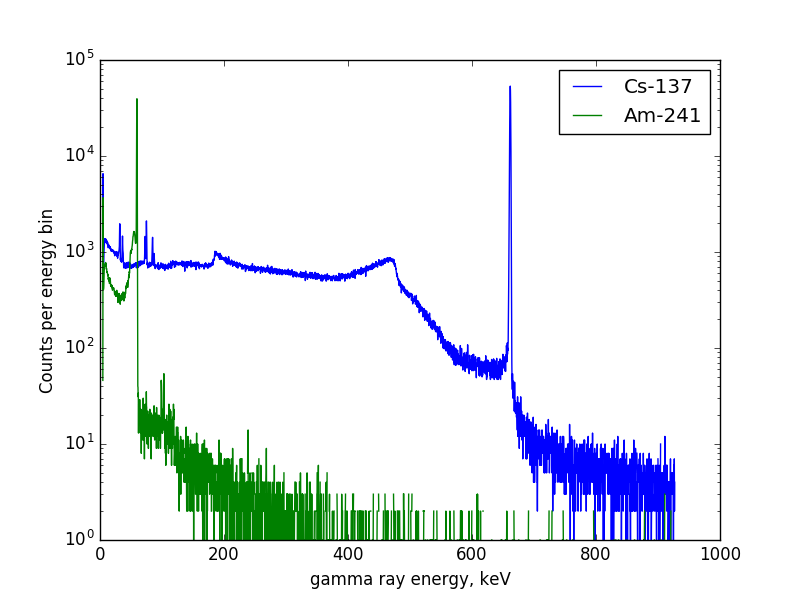
\includegraphics[width=0.7\textwidth]{cs_ba}
  \caption{This histogram is the result of applying the two-point calibration
  derived from the 59.5keV and 661.7keV photopeaks to the Cs and Am data. }
\label{fig:cesiumamericium}
\end{figure}

\begin{figure}[h]
  \centering
  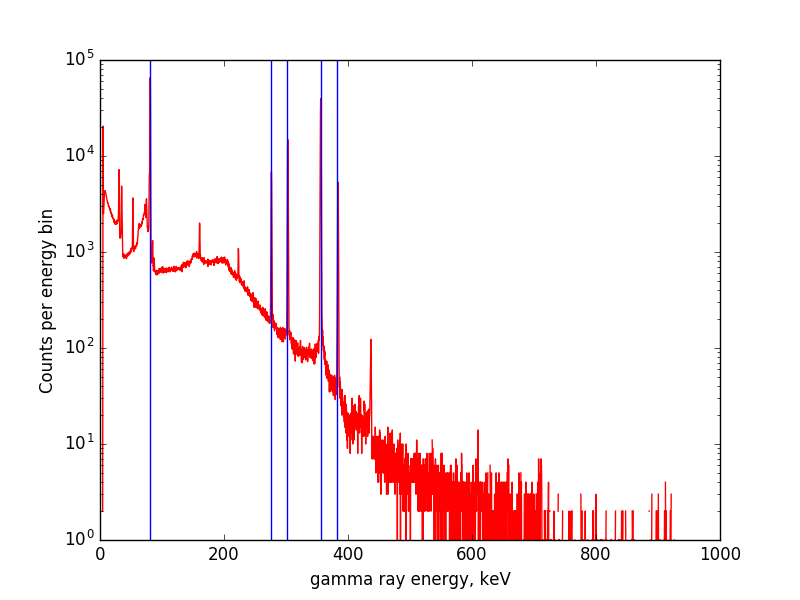
\includegraphics[width=0.7\textwidth]{Ba_data_check}
  \caption{Applying the two-point calibration to the Ba-133 data as shown above
  gives excellent agreement with data from NNDC on the energies of the
  gamma rays emitted in its decay (indicated by vertical lines). }
\label{fig:bariumcal}
\end{figure}
